% =====================================================================
% TLECUIL: A First-Order Fission Surface Power Sizer
% Theory, verification, benchmarks, and comparison with NASA EZ FSP Sizer
%
% Build:  latexmk -pdf tlecuil_theory.tex      (uses biber; see .latexmkrc)
% VS Code: LaTeX Workshop extension, recipe "latexmk (biber)" in
%          .vscode/settings.json
% Tables in benchmark_tables.tex are generated by ../benchmarks.py.
% =====================================================================
\documentclass[11pt]{article}
\usepackage[margin=1in]{geometry}
\usepackage[T1]{fontenc}
\usepackage{lmodern}
\usepackage{amsmath,amssymb}
\usepackage{booktabs,longtable,array,tabularx}
\usepackage{siunitx}
\usepackage{graphicx}
\usepackage{xcolor}
\usepackage[most]{tcolorbox}
\usepackage{placeins}
\usepackage{tikz}
\usetikzlibrary{arrows.meta,positioning,shapes.geometric}
\graphicspath{{figures/}}
\usepackage[style=ieee,backend=biber,doi=true,url=true,isbn=true]{biblatex}
\addbibresource{references.bib}
\usepackage[colorlinks=true,linkcolor=blue!50!black,citecolor=blue!50!black,urlcolor=blue!50!black]{hyperref}
\numberwithin{equation}{section}
\numberwithin{table}{section}
\sisetup{per-mode=symbol}

\newtcolorbox{assume}{colback=orange!6,colframe=orange!60!black,title=Assumption,fonttitle=\bfseries\small}
\newtcolorbox{code}{colback=blue!4,colframe=blue!50!black,title=In the code,fonttitle=\bfseries\small}
\newtcolorbox{physics}{colback=green!5,colframe=green!40!black,title=Physical meaning,fonttitle=\bfseries\small}
\newtcolorbox{keyidea}{colback=violet!5,colframe=violet!60!black,title=Key idea,fonttitle=\bfseries\small}
\newtcolorbox[auto counter]{tryit}[1][]{colback=yellow!7,colframe=yellow!50!black,title=Try it~\thetcbcounter,fonttitle=\bfseries\small,#1}
\newtcolorbox{review}{colback=gray!6,colframe=gray!60!black,title=Review note,fonttitle=\bfseries\small}

\newcommand{\tlecuil}{\textsc{Tlecuil}}
\newcommand{\Pdel}{P_\text{del}}
\newcommand{\Pconv}{P_\text{conv}}
\newcommand{\Pth}{P_\text{th}}

% AUTO-GENERATED by benchmarks.py -- do not edit by hand.
\newcommand{\etapcal}{0.756}
\newcommand{\errBtwo}{+2.5}
\newcommand{\errBthree}{+2.3}
\newcommand{\errBfour}{+15.3}
\newcommand{\idealmin}{13}
\newcommand{\idealmax}{24}
\newcommand{\sinkBtwo}{-3.0}
\newcommand{\sinkBthree}{-3.0}
\newcommand{\elecStirling}{44}
\newcommand{\elecBrayton}{28}
\newcommand{\elecStirlingPub}{25}
\newcommand{\elecBraytonPub}{13}
\newcommand{\tableradbench}{%
\begin{table}[ht]\centering\small
\caption{Main-radiator benchmark. Areas are total radiating area (both faces) including margin. B1 is used to calibrate $\eta_p$; B2--B4, not used in the calibration, are predicted with $\eta_p=\etapcal$ held fixed.}\label{tab:radbench}
\resizebox{\textwidth}{!}{\begin{tabular}{llrrrrrrr}\toprule
Case & Role & $Q$ (kW) & $T_\text{in}/T_\text{out}$ (K) & $T_s$ (K) & Published (m$^2$) & Ideal $\eta_p{=}1$ & Calibrated & Implied $\eta_p$\\\midrule
B1~\cite{fsp2010icd} & calibration & 140.0 & 420/390 & 250 & 185.0 & 139.9 (-24\%) & 185.0 (+0.0\%) & 0.756\\
B2~\cite{mason2025trades} & prediction & 119.0 & 433/403 & 270 & 140.0 & 108.5 (-23\%) & 143.5 (+2.5\%) & 0.775\\
B3~\cite{mason2025trades} & prediction & 180.0 & 504/379 & 270 & 180.0 & 139.2 (-23\%) & 184.1 (+2.3\%) & 0.773\\
B4~\cite{oleson2022deployable} & prediction & 126.4 & 420/370 & 185 & 133.4 & 116.3 (-13\%) & 153.8 (+15.3\%) & 0.872\\
\bottomrule\end{tabular}}\end{table}
}
\newcommand{\tablesysbench}{%
\begin{table}[ht]\centering\small
\caption{Electrical chain and first-law benchmark (acceptance $\pm5\%$). $P_\text{fix}$ is the fixed load assumed for the 2025 designs (an interpretation, see text). Rows marked $\dagger$ are identities by construction and are not counted as agreement.}\label{tab:sysbench}
\begin{tabular}{llcrrr}\toprule Case & Quantity & $P_\text{fix}$ (kWe) & Published & TLECUIL & Difference\\\midrule
S1~\cite{fsp2010icd} & Gross converter output (kWe)$^\dagger$ & -- & 48.0 & 48.0 & +0.0\%\\
S1~\cite{fsp2010icd} & Reactor thermal power (kWt) & -- & 186.0 & 184.6 & -0.7\%\\
S1~\cite{fsp2010icd} & Main radiator heat load (kWt) & -- & 140.0 & 136.6 & -2.4\%\\
S2~\cite{mason2025trades} & Gross converter output (kWe) & 2 & 50.4 & 50.2 & -0.4\%\\
S2~\cite{mason2025trades} & Main radiator heat load (kWt) & 2 & 119.0 & 124.1 & +4.3\%\\
S3~\cite{mason2025trades} & Gross converter output (kWe) & 2 & 46.7 & 46.4 & -0.5\%\\
S3~\cite{mason2025trades} & Main radiator heat load (kWt) & 2 & 180.0 & 182.3 & +1.3\%\\
S2~\cite{mason2025trades} & Gross converter output (kWe) & 0 & 50.4 & 48.2 & -4.4\%\\
S2~\cite{mason2025trades} & Main radiator heat load (kWt) & 0 & 119.0 & 119.1 & +0.1\%\\
S3~\cite{mason2025trades} & Gross converter output (kWe) & 0 & 46.7 & 44.4 & -4.8\%\\
S3~\cite{mason2025trades} & Main radiator heat load (kWt) & 0 & 180.0 & 174.4 & -3.1\%\\
\bottomrule\end{tabular}\end{table}
}
\newcommand{\tablescalebench}{%
\begin{table}[ht]\centering\small
\caption{Scaling benchmark against Table~V of \cite{mason2025trades}. TLECUIL is anchored only at 40\,kWe (same $\eta$ and PMAD efficiency) and predicts the other power levels with no fixed load and with a 2\,kWe fixed load. Implied $\eta$ is the efficiency NASA's numbers imply at each size.}\label{tab:scalebench}
\resizebox{\textwidth}{!}{\begin{tabular}{llrrrrrrrrr}\toprule Concept & kWe & kWt pub. & kWt ($P_\text{fix}{=}0$) & Diff. & kWt ($P_\text{fix}{=}2$) & Diff. & Implied $\eta$ & m$^2$ pub. & m$^2$ ($P_\text{fix}{=}2$) & Diff.\\\midrule
HP-Stirling & 10 & 49 & 42 & -14.6\% & 49 & -0.5\% & 0.287 & 40 & 39 & -2.0\%\\
 & 20 & 90 & 84 & -7.0\% & 91 & +0.7\% & 0.290 & 80 & 73 & -9.0\%\\
 & 40 & 175 & 167 & -4.4\% & 174 & -0.4\% & 0.287 & 140 & 140 & +0.0\%\\
 & 80 & 343 & 335 & -2.4\% & 342 & -0.4\% & 0.287 & 279 & 274 & -1.6\%\\
 & 100 & 429 & 418 & -2.5\% & 425 & -0.9\% & 0.286 & 351 & 342 & -2.7\%\\
\addlinespace
GC-Brayton & 10 & 72 & 55 & -24.0\% & 65 & -10.3\% & 0.182 & 57 & 51 & -10.9\%\\
 & 20 & 120 & 109 & -8.8\% & 119 & -0.6\% & 0.202 & 93 & 94 & +0.9\%\\
 & 40 & 230 & 219 & -4.8\% & 229 & -0.5\% & 0.202 & 180 & 180 & +0.0\%\\
 & 80 & 421 & 438 & +4.0\% & 448 & +6.3\% & 0.216 & 317 & 352 & +11.1\%\\
 & 100 & 517 & 547 & +5.8\% & 557 & +7.8\% & 0.219 & 380 & 438 & +15.4\%\\
\addlinespace
\bottomrule\end{tabular}}\end{table}
}
\newcommand{\tablecarnot}{%
\begin{table}[ht]\centering\small
\caption{Fraction of Carnot implied by published efficiencies, $f_C=\eta/(1-T_c/T_h)$. The value depends on how $T_h$ and $T_c$ are defined.}\label{tab:carnot}
\begin{tabular}{lrrrrr}\toprule Source & $\eta$ & $T_h$ (K) & $T_c$ (K) & $\eta_C$ & $f_C$\\\midrule
2010 reference, effective cycle temps~\cite{fsp2010icd} & 0.260 & 778 & 425 & 0.454 & 0.57\\
2025 HP-Stirling, hot/cold-end temps~\cite{mason2025trades} & 0.288 & 1050 & 420 & 0.600 & 0.48\\
2025 GC-Brayton, turbine inlet/cold end~\cite{mason2025trades} & 0.203 & 1100 & 390 & 0.645 & 0.31\\
Deployable concept, Stirling (700/150 C)~\cite{oleson2022deployable} & 0.261 & 973.15 & 423.15 & 0.565 & 0.46\\
TDU test, max power (NaK 875 K, water 350 K)~\cite{briggs2016tdu} & 0.233 & 875 & 350 & 0.600 & 0.39\\
SSE CTPC test, 12.5 kWe (1050 K / 525 K)~\cite{dhar1999sse} & 0.220 & 1050 & 525 & 0.500 & 0.44\\
\bottomrule\end{tabular}\end{table}
}
   % defines \etapcal and the benchmark tables

\title{\tlecuil{}: A First-Order Fission Surface Power Sizer\\[6pt]
\large Theory, verification, benchmarks against published NASA designs,\\
and comparison with the NASA EZ FSP Sizer}
\author{Irais Strong}
\date{Version 0.2.1 --- \today}

\begin{document}
\maketitle

\begin{abstract}
\tlecuil{} is an open, independent, first-order steady-state model of a fission
surface power (FSP) system. It walks the energy chain from the user bus back to
the reactor and returns reactor thermal power, conversion efficiency, waste-heat
loads, radiator areas and U-235 burned, for any delivered power. Every equation is
derived here from first principles and cited to primary sources. The code is
verified against hand calculations, conservation laws, closed-form limits and
numerical integration. It is then benchmarked against four published NASA designs
from 2010 to 2025. With an ideal radiator panel, \tlecuil{} underestimates
published radiator areas by \idealmin--\idealmax\,\%. A single panel-effectiveness
factor, calibrated on the 2010 reference design alone ($\eta_p=\etapcal$), reproduces
the two 2025 government designs, which were not used in the calibration, to within
3\,\%. Those designs were sized with NASA's EZ FSP Sizer, so this shows consistency
with NASA's sizing practice rather than independent physical validation. A third
design, from a different study, falls just outside the $\pm15\,\%$ acceptance band,
for reasons analysed here. Electrical-chain and first-law quantities agree to within
5\,\%. Section~\ref{sec:ez}
compares \tlecuil{} with NASA Glenn's EZ FSP Sizer and sets out where each is
the better tool. An AI-assisted review of v0.2 (IR-001) found no critical errors; its
findings are incorporated. Independent human review is planned (IR-002).
\end{abstract}

\tableofcontents

\section*{How to read this document (for students)}
\addcontentsline{toc}{section}{How to read this document (for students)}
This document is written so that an undergraduate in nuclear, mechanical or
aerospace engineering can follow every step.

\paragraph{What you need to know already.}
\begin{itemize}
  \item Calculus I--II: derivatives, integrals, and integration by partial fractions.
  \item Introductory thermodynamics: the first law (energy is conserved) and the
        second law (heat engines cannot convert all heat to work).
  \item Introductory heat transfer: what thermal radiation is. Section~\ref{sec:primer}
        reviews everything else you need.
\end{itemize}

\paragraph{How to read it.}
\begin{enumerate}
  \item Read Section~\ref{sec:primer} first. It explains the physics in words, with no
        derivations.
  \item On a first pass through Sections~\ref{sec:power}--\ref{sec:opt}, read the
        \emph{Key idea} boxes and the equations in boxes, and skip the derivations.
        Come back to the derivations on a second pass.
  \item Do the \emph{Try it} exercises. Answers are in Appendix~\ref{app:answers}.
  \item The worked example (Section~\ref{sec:worked}) runs one complete case by hand.
        Reproduce it with a calculator, then with \texttt{python tlecuil.py}.
  \item Unfamiliar words are defined in the glossary (Appendix~\ref{app:glossary}).
\end{enumerate}

\paragraph{One notation rule.} Engineers write kWe for \emph{electrical} kilowatts and
kWt for \emph{thermal} kilowatts. Both are kilowatts, i.e.\ kilojoules per second. The
letter only says which kind of energy is flowing.

%=====================================================================
\section{Introduction}\label{sec:intro}
%=====================================================================

\subsection{Purpose}
A planetary-surface fission power system converts fission heat to electricity and
must reject most of that heat by thermal radiation. A first-order sizer answers
three linked questions. How much heat must the reactor produce to deliver $\Pdel$
to users? How much heat must be rejected, and at what temperature? How much
radiating area does that take?

NASA's FSP reference designs have been sized for 40\,kWe net
\cite{fsp2010icd,mason2025trades}. NASA's 2025 solicitation moved to a system of
at least 100\,kWe with closed-Brayton conversion \cite{nasa2025fsp}, and the
government design used in recent radiation studies is a 500\,kWt, 100\,kWe
Brayton system \cite{wilson2026dose}. \tlecuil{} has no upper power limit
(Section~\ref{sec:scaling}).

\subsection{The name}
\emph{Tlecuilli} (Nahuatl) is the three-stone hearth: a fire pit with three
stones that support the cooking vessel \cite{karttunen1992}. Molina's 1571
dictionary renders it \emph{hogar}, both hearth and home \cite{wired_tlecuilli}. The
three stones stand for the three subsystems this model balances: the reactor (the
fire), power conversion (the vessel it heats), and heat rejection (the heat that
must leave).

\subsection{What \tlecuil{} is and is not}
\tlecuil{} is a thermal--electrical balance built only from first-principles physics
and inputs the user supplies. It does \emph{not} model component masses,
shielding, dose, reactor physics or transients, and it contains no proprietary or
hardware-specific correlations. It is not a re-implementation of NASA's EZ FSP
Sizer, which combines first-order physics with hardware-based curve fits and mass
models \cite{mason2025trades} (Section~\ref{sec:ez}).

\subsection{How to read this document}
Each section maps to a numbered block in \texttt{tlecuil.py}. ``In the code''
boxes name the implementing function, so the math and the code can be checked line
by line. ``Review note'' boxes flag judgement calls a reviewer should check.
Benchmark tables are generated by \texttt{benchmarks.py} and \verb|\input| into
this document, so the tables always show what the code computes.

\subsection{Revision history}
\begin{center}
\begin{tabular}{lp{0.78\textwidth}}
\toprule
Version & Change\\
\midrule
0.1 & First draft (as \texttt{fsp\_sizer.py}).\\
0.2 & Renamed \tlecuil{}. \textbf{Corrected an error in v0.1}: v0.1 divided by the
number of radiating sides twice. The value it labelled ``emitting area'' was in fact
the panel planform, half the true total radiating area for two-sided panels, and the
value it labelled ``planform'' was half the true planform. Also fixed a round-off
error in the fluid-loop integral for sink temperatures near 0\,K, found by an
AI-assisted review (IR-001). Added fixed parasitic loads, reactor heat losses, panel
effectiveness, area margin, citations, benchmarks, and the EZ FSP Sizer
comparison. A regression test now guards the correction.\\
\bottomrule
\end{tabular}
\end{center}

%=====================================================================
\section{Background: the physics behind a fission surface power system}\label{sec:primer}
%=====================================================================

\subsection{What the system is}
A fission surface power (FSP) system is a small nuclear power plant set on the surface
of the Moon or Mars. Figure~\ref{fig:block} follows the energy through it, using the
numbers from the worked example in Section~\ref{sec:worked}.
\begin{enumerate}
  \item The \textbf{reactor} splits uranium atoms (fission) and turns their energy into
        heat. A liquid metal or gas carries the heat away.
  \item The \textbf{power converter}, a Stirling or Brayton engine, turns part of that heat
        into electricity, as a car engine turns part of the fuel's heat into motion.
  \item The \textbf{radiator}, a set of large panels, gets rid of the heat the engine could
        not use.
  \item \textbf{PMAD} (power management and distribution) conditions the electricity and
        sends it, often through a cable about a kilometre long, to the users.
\end{enumerate}

\begin{figure}[ht]
\centering
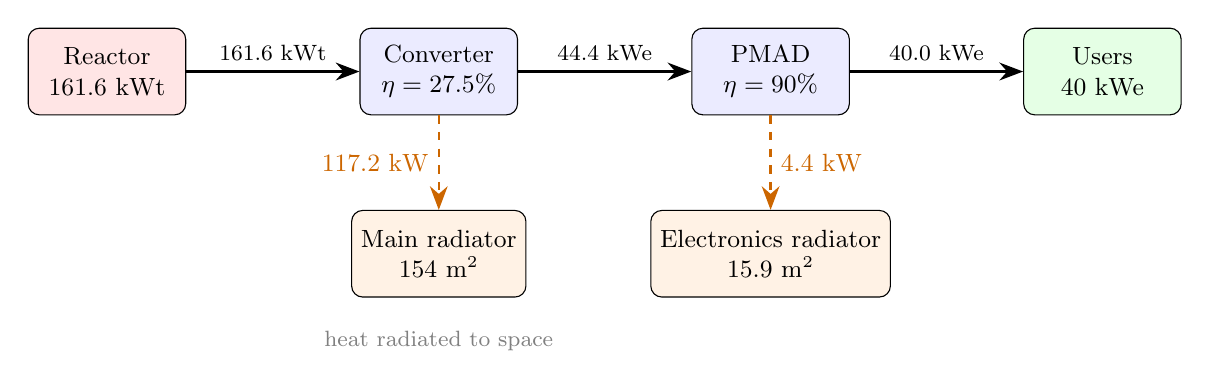
\begin{tikzpicture}[
  box/.style={draw, rounded corners, align=center, minimum width=2.0cm, minimum height=1.1cm, fill=#1},
  box/.default=blue!8,
  flow/.style={-{Stealth[length=3mm]}, very thick},
  heat/.style={-{Stealth[length=3mm]}, thick, orange!80!black, dashed},
  font=\small, every edge quotes/.style={font=\footnotesize}]
\node[box=red!10]   (R) {Reactor\\161.6 kWt};
\node[box, right=2.2cm of R] (C) {Converter\\$\eta=27.5\%$};
\node[box, right=2.2cm of C] (P) {PMAD\\$\eta=90\%$};
\node[box=green!10, right=2.2cm of P] (U) {Users\\40 kWe};
\draw[flow] (R) -- node[above, font=\footnotesize]{161.6 kWt} (C);
\draw[flow] (C) -- node[above, font=\footnotesize]{44.4 kWe} (P);
\draw[flow] (P) -- node[above, font=\footnotesize]{40.0 kWe} (U);
\node[box=orange!10, below=1.2cm of C] (MR) {Main radiator\\154 m$^2$};
\node[box=orange!10, below=1.2cm of P] (ER) {Electronics radiator\\15.9 m$^2$};
\draw[heat] (C) -- node[left]{117.2 kW} (MR);
\draw[heat] (P) -- node[right]{4.4 kW} (ER);
\node[below=0.3cm of MR, font=\footnotesize, text=gray] {heat radiated to space};
\end{tikzpicture}
\caption{Energy flow through the default 40\,kWe system. Solid arrows are useful power;
dashed arrows are waste heat that must be radiated away. Every kilowatt that enters on
the left leaves somewhere on the right: $161.6 = 40.0 + 117.2 + 4.4$.}
\label{fig:block}
\end{figure}

\subsection{Power and energy}
\emph{Energy} is measured in joules (J). \emph{Power} is energy per unit time:
1\,watt = 1\,J/s, and 1\,kW = 1000\,J/s. This document works almost entirely with power,
because the system runs steadily for years. A 40\,kWe system delivers 40\,000\,J of
electrical energy every second.

\subsection{Conservation of energy (the first law)}
Energy cannot be created or destroyed. In steady operation, the power flowing into any
component equals the power flowing out. Think of a budget: the reactor is the income, and
every kilowatt has to be spent somewhere, either as electricity for the users or as heat
that is thrown away. TLECUIL checks this budget on every run (Section~\ref{sec:elec}).

\subsection{Why an engine must throw heat away (the second law)}
Sadi Carnot compared a heat engine to a water wheel. Water falling from a high level to
a low level turns the wheel, but the water has to go somewhere at the bottom. Heat
``falling'' from a hot temperature $T_h$ to a cold temperature $T_c$ drives the engine,
and some heat always has to be released at the cold side. The best any engine can do is
the Carnot efficiency $1-T_c/T_h$, with temperatures in kelvin. For $T_h=850$\,K and
$T_c=425$\,K that is 50\,\%. Real engines reach roughly half of that
(Section~\ref{sec:eta}). The rest of the heat, about three quarters of what the reactor
makes, must be rejected.

\subsection{Getting rid of heat in a vacuum}
On Earth, power plants dump waste heat into rivers or cooling towers, using conduction
and convection to water or air. The Moon has no air and no water, so the only way to
lose heat is \emph{thermal radiation}: every warm surface emits infrared light. A perfect
emitter (a ``black body'') at temperature $T$ radiates $\sigma T^4$ watts per square metre,
where $\sigma=5.67\times10^{-8}$\,W\,m$^{-2}$\,K$^{-4}$ is the Stefan--Boltzmann constant.
Real surfaces emit a fraction $\varepsilon$ (the \emph{emissivity}) of that.

The fourth power is the most important fact in this document. Doubling the radiator
temperature multiplies the heat it can radiate by $2^4=16$ (Figure~\ref{fig:flux}). That
is why space radiators run as hot as the engine allows, and why radiator area is a
central part of FSP design.

The radiator also \emph{receives} radiation from the Sun, the warm lunar soil and cold
deep space. Rather than track each source, we lump them into one \emph{effective sink
temperature} $T_s$: the radiator behaves as if it faced a single surrounding at $T_s$.

\begin{figure}[ht]
\centering
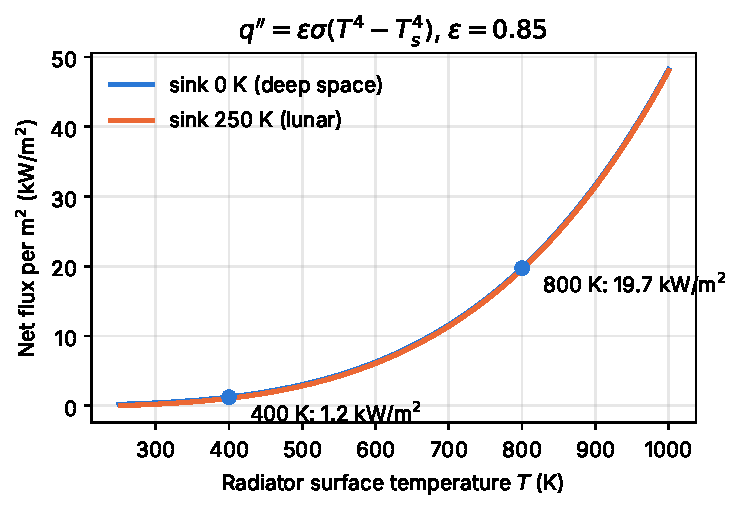
\includegraphics[width=0.62\textwidth]{flux_vs_T.pdf}
\caption{Net heat radiated per square metre of surface. Going from 400\,K to 800\,K
multiplies the flux by 16. A warmer sink (orange) reduces the net flux, most of all at low
radiator temperatures.}
\label{fig:flux}
\end{figure}

\subsection{Where the heat comes from}
Each fission of a uranium-235 nucleus releases about 200\,MeV ($3.2\times10^{-11}$\,J)
that can be turned into heat \cite{lamarsh2017}. That is tiny per atom, but a gram of
U-235 holds about $2.6\times10^{21}$ atoms. The default 162\,kWt reactor fissions only about
0.17\,g of uranium per day (Section~\ref{sec:fuel}). This energy density is why fission is
attractive where solar power fails, such as during the 14-day lunar night.

\subsection{What ``first-order'' means}
A \emph{first-order} model keeps only the physics that sets the answer to within
roughly 10--30\,\% and leaves out the details. TLECUIL captures energy conservation, the
heat-engine limit and radiation. It ignores, for example, how the radiator panels are
built, how temperatures change from day to night, and how much each part weighs. Models
like this are used early in a design, to compare options quickly before anyone builds
detailed models.

\begin{keyidea}
An FSP system is an energy budget. The reactor supplies heat; the engine turns about a
quarter of it into electricity; and almost everything else must be radiated away, at a
rate that grows as the fourth power of temperature.
\end{keyidea}

%=====================================================================
\section{Electrical chain}\label{sec:power}
%=====================================================================

\begin{keyidea}
Start from what the users need and work backward. Every loss between the converter and
the users, including power used by the plant itself, means the converter, and so the
reactor, must produce more.
\end{keyidea}

\subsection{Definitions}
\begin{itemize}
  \item $\Pdel$: power delivered to the user bus (kWe), the requirement.
  \item $\Pconv$: gross electrical output at the converter terminals (kWe).
  \item $f_\text{par}$: fraction of $\Pconv$ used by loads that scale with power (pumps).
  \item $P_\text{fix}$: loads that do not scale with power (housekeeping,
        instruments). \textcite{mason2025trades} allow up to 2\,kWe.
  \item $\eta_\text{PMAD}$: power management and distribution efficiency, bus power
        divided by PMAD input. It lumps conditioning, conversion and cable losses.
        Published values are about 0.90 for Brayton and 0.83 for Stirling
        \cite{mason2025trades}, and 0.87 in \cite{oleson2022deployable}.
\end{itemize}

\subsection{Derivation}
Parasitic loads are taken from the converter output first. PMAD then delivers a
fraction $\eta_\text{PMAD}$ of what remains:
\begin{equation}
  P_\text{par} = f_\text{par}\Pconv + P_\text{fix},
  \label{eq:ppar}
\end{equation}
\begin{equation}
  \Pdel = \eta_\text{PMAD}\left[(1-f_\text{par})\Pconv - P_\text{fix}\right]
  \;\Longrightarrow\;
  \Pconv = \frac{\Pdel/\eta_\text{PMAD} + P_\text{fix}}{1-f_\text{par}},
  \label{eq:pconv}
\end{equation}
\begin{equation}
  L_\text{PMAD} = (\Pconv - P_\text{par}) - \Pdel .
  \label{eq:lpmad}
\end{equation}

\begin{physics}
The requirement is fixed at the bus, and every upstream loss inflates what the
converter, and so the reactor, must produce. The fixed load $P_\text{fix}$ matters
mostly for small systems. Section~\ref{sec:bench} shows that a fixed load of about
2\,kWe makes NASA's published Stirling designs consistent with a single conversion
efficiency from 10 to 100\,kWe.
\end{physics}

\begin{assume}
All parasitic power and all PMAD losses end up as low-temperature heat in the
electronics and are rejected by the electronics radiator (Section~\ref{sec:elec}).
In reality some pump work heats the coolant. Sending it to the colder radiator is
conservative for \emph{total} radiator area, because a colder radiator needs more area
per kilowatt. It slightly under-loads the main radiator.
\end{assume}

\paragraph{Reading Eq.~\eqref{eq:pconv} step by step.} Divide $\Pdel$ by
$\eta_\text{PMAD}$ to find what must \emph{enter} PMAD. Add the fixed load $P_\text{fix}$.
Then divide by $(1-f_\text{par})$, because the proportional loads take their share of
everything the converter makes. Example: with $\Pdel=40$\,kWe, $\eta_\text{PMAD}=0.90$ and no
parasitic loads, $\Pconv = 40/0.90 = 44.4$\,kWe.

\begin{code}
\texttt{size\_fsp()}, lines marked ``Theory eq.~\ref{eq:pconv}'' and ``eq.~\ref{eq:lpmad}''.
\end{code}

\begin{tryit}[label=try:pconv]
A 100\,kWe system has $\eta_\text{PMAD}=0.90$, $f_\text{par}=0$ and a 2\,kWe fixed load. What
gross power must the converter produce? How much of it is lost in PMAD?
\end{tryit}

%=====================================================================
\section{Power conversion}\label{sec:eta}
%=====================================================================

\begin{keyidea}
Conversion efficiency decides how much heat must be thrown away. Lower efficiency means
a bigger reactor \emph{and} a bigger radiator for the same electrical output.
\end{keyidea}

\subsection{First law around the converter}
In steady state the converter takes heat $Q_\text{in}$, produces $\Pconv$ of
electricity, and rejects the rest:
\begin{equation}
  Q_\text{in} = \Pconv + Q_\text{conv}.
  \label{eq:firstlaw}
\end{equation}
With conversion efficiency $\eta \equiv \Pconv/Q_\text{in}$,
\begin{equation}
  Q_\text{in} = \frac{\Pconv}{\eta}, \qquad
  Q_\text{conv} = \Pconv\,\frac{1-\eta}{\eta}.
  \label{eq:qin}
\end{equation}

\begin{physics}
$(1-\eta)/\eta$ is the heat rejected per unit of electricity. At $\eta=0.25$ it
is 3: each kilowatt of electricity costs three kilowatts of waste heat. This is
why efficiency and radiator size are so tightly coupled.
\end{physics}

\subsection{The second law and the Carnot limit}
For any engine between absolute temperatures $T_h$ and $T_c$ \cite{smith2001thermo},
\begin{equation}
  \eta \le \eta_C = 1 - \frac{T_c}{T_h}.
  \label{eq:carnot}
\end{equation}
A reversible engine generates no entropy, so the entropy taken in,
$Q_\text{in}/T_h$, equals the entropy rejected, $Q_\text{conv}/T_c$. That gives
$Q_\text{conv}/Q_\text{in} = T_c/T_h$, and Eq.~\eqref{eq:carnot} follows. Any
irreversibility adds entropy and therefore rejects more heat. In fixed-efficiency
mode the code refuses any $\eta>\eta_C$.

\subsection{Fraction-of-Carnot model}
\begin{equation}
  \eta = f_C\left(1-\frac{T_c}{T_h}\right), \qquad 0<f_C\le 1 .
  \label{eq:fc}
\end{equation}
Table~\ref{tab:carnot} lists the $f_C$ implied by published designs and tests.
It ranges from about 0.31 for the 2025 Brayton design to 0.57 for the 2010
Stirling reference.

\begin{review}
$f_C$ is \emph{not portable} unless $T_h$ and $T_c$ are defined the same way. The
2010 design quotes effective \emph{cycle} temperatures (778/425\,K), which gives
$f_C=0.57$ \cite{fsp2010icd}. The Technology Demonstration Unit test quotes
\emph{fluid} temperatures (875\,K NaK, 350\,K water), which gives $f_C=0.39$
\cite{briggs2016tdu}. Heat-exchanger temperature drops sit between the two
definitions. Users should take $f_C$ from a source that uses the same temperature
definition as their inputs.
\end{review}

\subsection{Reactor-to-converter heat losses}\label{sec:loss}
Some reactor heat never reaches the converter: radial leakage, and losses from the
reactor vessel and piping. \textcite{oleson2022deployable} report 18\,\% reactor
losses and 2\,\% from reactor to Stirling hot end for a heat-pipe design. With a
loss fraction $f_\text{loss}$,
\begin{equation}
  \Pth = \frac{Q_\text{in}}{1-f_\text{loss}}, \qquad Q_\text{loss} = \Pth - Q_\text{in}.
  \label{eq:loss}
\end{equation}
$Q_\text{loss}$ leaves through the reactor and shield surfaces and is not counted in
the main radiator. The default is $f_\text{loss}=0$.

\begin{code}
\texttt{conversion\_efficiency()}; second-law guard in \texttt{validate()}; Eq.~\eqref{eq:loss} in \texttt{size\_fsp()}.
\end{code}

\begin{tryit}[label=try:eta]
How many kilowatts of waste heat does each kilowatt of electricity cost at $\eta=0.20$?
At $\eta=0.30$? By what factor does the radiator heat load change between the two?
\end{tryit}

%=====================================================================
\section{Main heat-rejection radiator}\label{sec:rad}
%=====================================================================

\begin{keyidea}
Radiator area $=$ heat to reject $\div$ heat each square metre can radiate. The second
number depends on $T^4$, so small temperature changes make large area changes.
\end{keyidea}

\subsection{Net radiative flux}
A gray, diffuse surface at $T$ facing surroundings that can be lumped into an
effective sink temperature $T_s$ rejects a net flux
\cite{howell2021radiation,gilmore2002thermal}
\begin{equation}
  q'' = \varepsilon\sigma\left(T^4 - T_s^4\right)\quad[\si{W/m^2}~\text{of radiating surface}],
  \label{eq:flux}
\end{equation}
with $\sigma = \SI{5.670374419e-8}{W.m^{-2}.K^{-4}}$ \cite{codata2018}. $T_s$ is
where the environment enters. On the Moon, the sink seen by a fixed vertical radiator
varies from about 100 to 200\,K at the south pole and from 100 to 320\,K at the
equator \cite{mason2025trades}.

\subsection{Area definitions}
Eq.~\eqref{eq:flux} is per square metre of \emph{radiating surface}. A two-sided
panel has two radiating faces, so
\begin{equation}
  A_\text{planform} = \frac{A}{n_\text{sides}} .
  \label{eq:planform}
\end{equation}
NASA FSP studies quote the total of both faces. The 2010 design quotes ``total
two-sided'' area \cite{fsp2010icd}, and the 2025 design counts each
\SI{2}{m}$\times$\SI{2.5}{m} panel as \SI{10}{m^2} \cite{mason2025trades}.
\tlecuil{} therefore reports $A$, the total radiating area, as its primary
result. Version 0.1 had this wrong (see the revision history).

\subsection{Panel effectiveness}\label{sec:etap}
A real panel does not radiate at the coolant temperature. Heat passes through a
heat pipe or tube wall, a saddle and a facesheet, and the facesheet cools away from
the heat pipe (fin efficiency). Space-radiator models commonly multiply the
radiated flux by a fin-efficiency factor \cite{wang2021entropy,gilmore2002thermal}.
\tlecuil{} uses one panel effectiveness $\eta_p\in(0,1]$ that lumps fin efficiency,
the conduction drops, and any shortfall in the assumed view factor:
\begin{equation}
  k \equiv \eta_p\,\varepsilon\,\sigma .
  \label{eq:k}
\end{equation}

\begin{review}
$\eta_p$ is a \emph{calibration factor}, not a measured property. The default
($\eta_p=0.76$) is back-calculated from one published design (B1,
Section~\ref{sec:bench}) and then tested against independent designs. A detailed
panel model (heat-pipe $\Delta T$, fin equation, view factors to terrain) would
replace it, and is listed as future work.
\end{review}

\subsection{Radiator temperatures}
\begin{equation}
  T_\text{in} = T_c - \Delta T_\text{HX}, \qquad T_\text{out} = T_\text{in} - \Delta T_\text{rad}.
  \label{eq:tin}
\end{equation}
For the 2010 design, $T_c=425$\,K and the water loop runs from 420 to 390\,K
\cite{fsp2010icd}.

\subsection{Case (a): isothermal radiator}
\begin{equation}
  A = (1+m)\,\frac{Q_\text{conv}}{k\left(T_\text{in}^4 - T_s^4\right)},
  \label{eq:aiso}
\end{equation}
where $m$ is the area margin. NASA studies use $m=0.10$ \cite{fsp2010icd,mason2025trades}.

\subsection{Case (b): pumped fluid loop}
In a pumped loop the coolant cools as it radiates. For a strip $\mathrm{d}A$ where
the coolant is at $T$, energy lost by the fluid equals energy radiated:
\begin{equation}
  -\dot m c_p\,\mathrm{d}T = k\left(T^4 - T_s^4\right)\mathrm{d}A .
  \label{eq:strip}
\end{equation}
Separating variables and integrating from outlet to inlet, with
$\dot m c_p = Q_\text{conv}/(T_\text{in}-T_\text{out})$:
\begin{equation}
  A = (1+m)\,\frac{\dot m c_p}{k}\int_{T_\text{out}}^{T_\text{in}}\frac{\mathrm{d}T}{T^4 - T_s^4}.
  \label{eq:afluid}
\end{equation}

Figure~\ref{fig:profile} shows how the coolant temperature falls along a radiator with a
large temperature drop. It does not fall in a straight line. The hot inlet end radiates
far more strongly ($T^4$ again), so the coolant cools fastest there.

\begin{figure}[ht]
\centering
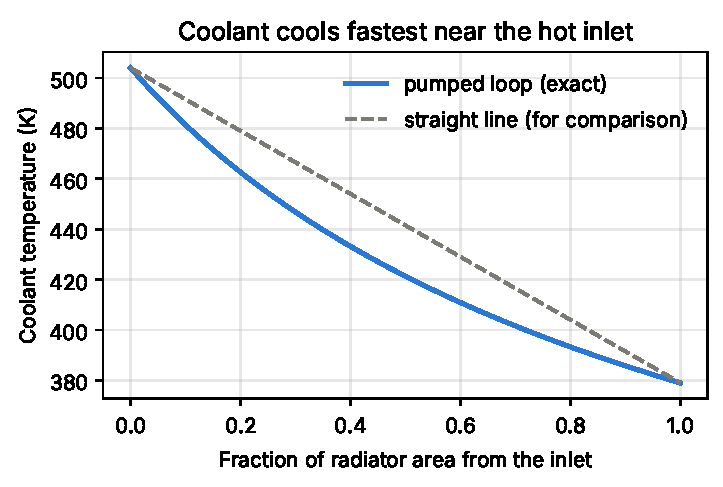
\includegraphics[width=0.6\textwidth]{fluid_loop_profile.pdf}
\caption{Coolant temperature along a pumped-loop radiator, from Eq.~\eqref{eq:afluid}, for the
2025 Brayton loop (504$\to$379\,K, $T_s=270$\,K). For the same heat load, this radiator needs
about twice the area of an ideal isothermal radiator at the inlet temperature.}
\label{fig:profile}
\end{figure}

\paragraph{Closed-form integral.}
With $a=T_s$, factor the denominator as a difference of squares,
$T^4-a^4=(T^2-a^2)(T^2+a^2)$. Partial fractions then split the integrand into two simple
pieces:
\[
\frac{1}{T^4-a^4} = \frac{1}{2a^2}\left[\frac{1}{T^2-a^2}-\frac{1}{T^2+a^2}\right].
\]
(Check it: put the bracket over a common denominator. The numerator is
$(T^2+a^2)-(T^2-a^2)=2a^2$.) Each piece has a standard integral,
$\int\frac{\mathrm{d}T}{T^2-a^2}=\frac{1}{2a}\ln\frac{T-a}{T+a}$ and
$\int\frac{\mathrm{d}T}{T^2+a^2}=\frac{1}{a}\arctan\frac{T}{a}$, which together give
\begin{equation}
  F(T) = \frac{1}{4a^3}\ln\frac{T-a}{T+a} - \frac{1}{2a^3}\arctan\frac{T}{a},
  \qquad T>a>0,
  \label{eq:antider}
\end{equation}
so the integral is $F(T_\text{in})-F(T_\text{out})$. For $a=0$ the integrand is
$T^{-4}$ and $F(T)=-1/(3T^3)$. (Eq.~\eqref{eq:antider} itself does not reduce to that
form as $a\to0$. Its two terms grow like $a^{-3}$ and largely cancel.)

\paragraph{Numerical evaluation.} That cancellation makes Eq.~\eqref{eq:antider}
inaccurate when $a\ll T$: in double precision it returns a negative area at
$a=10^{-3}$\,K. For $a<T_\text{out}/2$ the code instead uses the convergent series
\begin{equation}
  \int_{T_\text{out}}^{T_\text{in}}\frac{\mathrm{d}T}{T^4-a^4}
  = \sum_{k=0}^{\infty}\frac{a^{4k}}{4k+3}\left(T_\text{out}^{-(4k+3)} - T_\text{in}^{-(4k+3)}\right),
  \label{eq:series}
\end{equation}
obtained by expanding $1/(T^4-a^4)=\sum_k a^{4k}/T^{4k+4}$. Each term is at most 1/16
of the previous, so 20 terms reach machine precision. Both branches are checked
against numerical quadrature for sinks from $10^{-9}$ to 290\,K.

\begin{physics}
For the same inlet temperature, a fluid loop needs more area than an isothermal
radiator, because its downstream end is cooler. As $\Delta T_\text{rad}\to0$,
Eq.~\eqref{eq:afluid} reduces to Eq.~\eqref{eq:aiso}. Both limits are checked in the
test suite.
\end{physics}

\begin{tryit}[label=try:rad]
An ideal isothermal radiator ($\eta_p=1$, $\varepsilon=0.85$, $T_s=0$, no margin) must reject
100\,kW. Find its area at $T=400$\,K and at $T=500$\,K. Explain the ratio using $T^4$.
\end{tryit}

\begin{code}
\texttt{radiating\_area\_m2()} implements Eqs.~\eqref{eq:aiso}--\eqref{eq:afluid}
(margin is applied in \texttt{size\_fsp()}); \texttt{\_integral\_inv\_t4()} chooses
between Eq.~\eqref{eq:antider} (\texttt{\_antiderivative()}) and Eq.~\eqref{eq:series}.
\end{code}

%=====================================================================
\section{Electronics radiator and the energy balance}\label{sec:elec}
%=====================================================================
Electronics must run cool, so their heat goes to a separate radiator. Its
temperature is 333\,K in \cite{mason2025trades}. The heat is
\begin{equation}
  Q_\text{elec} = L_\text{PMAD} + P_\text{par},
  \label{eq:qelec}
\end{equation}
rejected by an isothermal radiator at $T_e$ (Eq.~\eqref{eq:aiso} with $T_e$). Every
kilowatt the reactor makes must leave as bus power or as heat:
\begin{equation}
  \Pth = \Pdel + Q_\text{conv} + Q_\text{elec} + Q_\text{loss}.
  \label{eq:balance}
\end{equation}
Eq.~\eqref{eq:balance} follows algebraically from the earlier equations, so its
residual, computed on every run, checks the \emph{implementation} (no term dropped or
double counted), not the physics.

%=====================================================================
\section{Fuel burned}\label{sec:fuel}
%=====================================================================
Each U-235 fission releases about $E_f\approx200$\,MeV of recoverable energy
\cite{lamarsh2017}. Over $t$ full-power years the mass fissioned is
\begin{equation}
  \dot N_f = \frac{\Pth}{E_f}, \qquad m_f = \frac{\dot N_f\,t}{N_A}\,M_{235},
  \label{eq:mf}
\end{equation}
which is about \SI{1.05}{g} per MWd. The U-235 \emph{consumed} is larger by
$(1+\alpha)$, where $\alpha$ is the capture-to-fission ratio. Neither is the core
\emph{loading}, which is set by criticality and must come from transport
calculations.

\begin{tryit}[label=try:fuel]
How much U-235 does a 400\,kWt reactor fission in 10 full-power years? Use the
1.05\,g/MWd rule and check it with \texttt{python tlecuil.py}.
\end{tryit}

%=====================================================================
\section{Cold-end temperature that minimises radiator area}\label{sec:opt}
%=====================================================================
\begin{keyidea}
Running the engine's cold side hotter shrinks the radiator but wastes more heat. There is
a temperature where the radiator is smallest, but that is not where the whole system is
lightest.
\end{keyidea}

Raising $T_c$ raises the radiator temperature, so flux grows as $T^4$, but it also
lowers $\eta$ (Eq.~\eqref{eq:fc}), so the heat load grows. Between those effects lies
an area minimum (Figure~\ref{fig:tctrade}).

\begin{figure}[ht]
\centering
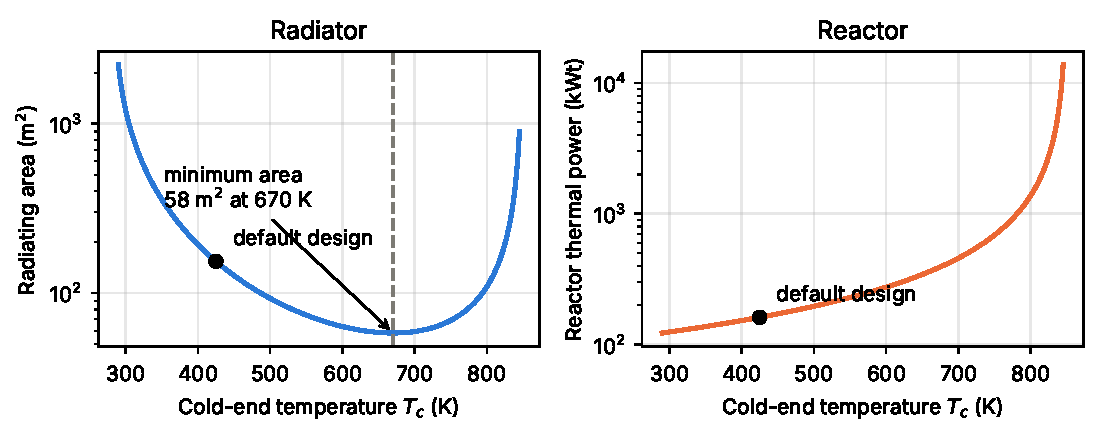
\includegraphics[width=\textwidth]{tc_trade.pdf}
\caption{The central trade for the default design, computed by TLECUIL. Left: radiator area
has a minimum. Right: reactor power keeps rising as $T_c$ rises, because efficiency falls.
The default design (dot) sits well below the area minimum, as real designs do.}
\label{fig:tctrade}
\end{figure} For $T_s=0$, no temperature drops and an isothermal radiator, with
$\tau=T_c/T_h$:
\begin{equation}
  A\propto g(\tau) = \frac{1-f_C(1-\tau)}{f_C(1-\tau)\,\tau^4}.
\end{equation}
To find the minimum, differentiate and set the derivative to zero. It is easier to
differentiate $\ln g$, which has its minimum at the same place, because logarithms turn
products and quotients into sums:
\[
\ln g = \ln\bigl(1-f_C+f_C\tau\bigr) - \ln f_C - \ln(1-\tau) - 4\ln\tau,
\qquad
\frac{\mathrm{d}\ln g}{\mathrm{d}\tau} = \frac{f_C}{1-f_C+f_C\tau}+\frac{1}{1-\tau}-\frac{4}{\tau}=0 .
\]
Multiplying through by $\tau(1-\tau)(1-f_C+f_C\tau)$ and collecting powers of $\tau$ gives
a quadratic:
\begin{equation}
  4f_C\tau^2 + (5-8f_C)\tau - 4(1-f_C) = 0
  \;\Longrightarrow\;
  \tau^* = \frac{-(5-8f_C)+\sqrt{(5-8f_C)^2+64f_C(1-f_C)}}{8f_C}.
  \label{eq:tauopt}
\end{equation}
For $f_C=1$ this gives the classic $\tau^*=3/4$, derived for space nuclear power
radiators by \textcite{bucher1960} and also posed as a textbook exercise
\cite{smith2001thermo}. For $f_C=0.5$ it gives $\tau^*=0.78$. That is consistent
with the 0.75--0.80 range for minimum radiator area reported in the NASA megawatt-class
space power study \cite{wetch1988mcnsps}. With a
non-zero sink, temperature drops or a fluid loop there is no closed form, so the
code uses a golden-section search and checks it against Eq.~\eqref{eq:tauopt}.

\begin{tryit}[label=try:opt]
Set $f_C=1$ in Eq.~\eqref{eq:tauopt} and show that $\tau^*=3/4$. Then put $\tau=3/4$ back into
the derivative above and check that it equals zero.
\end{tryit}

\begin{physics}
\textbf{Minimum radiator area is not minimum system mass.} At the area optimum the
efficiency is low and the reactor is large. NASA's design temperatures sit well below
the area optimum because the reactor, shield and converter mass also count
\cite{mason2025trades}. Mass is outside \tlecuil{}'s scope (Section~\ref{sec:limits}).
\end{physics}

%=====================================================================
\section{Scaling with power}\label{sec:scaling}
%=====================================================================
With fixed efficiencies and temperatures and $P_\text{fix}=0$, every heat and power
quantity, and so every area, is proportional to $\Pdel$. A non-zero $P_\text{fix}$
makes small systems relatively more expensive. There is no mathematical limit at
40 or 100\,kWe. The real limits are engineering ones that enter through the inputs:
converter unit size and efficiency, radiator packaging, reactor criticality and
shielding. Section~\ref{sec:bench} shows where the constant-efficiency assumption
fails.

%=====================================================================
\section{Worked example: default 40\,kWe case}\label{sec:worked}
%=====================================================================
This section runs one complete case by hand. Every number matches the output of
\texttt{python tlecuil.py}.

\paragraph{Inputs} (generic, not a specific NASA design):
$\Pdel=40$\,kWe, $\eta_\text{PMAD}=0.90$, no parasitic loads, $f_C=0.55$, $T_h=850$\,K,
$T_c=425$\,K, a 5\,K heat-exchanger drop, a water loop from 420 to 390\,K, $T_s=250$\,K,
$\varepsilon=0.85$, $\eta_p=0.76$, $m=0.10$, $T_e=333$\,K, 10 full-power years.

\paragraph{Step 1: converter output} (Eq.~\eqref{eq:pconv}).
$\Pconv = 40/0.90 = 44.44$\,kWe. PMAD loses $44.44-40 = 4.44$\,kW as heat.

\paragraph{Step 2: efficiency} (Eq.~\eqref{eq:fc}).
Carnot: $1-425/850 = 0.50$. Real engine: $\eta = 0.55\times0.50 = 0.275$.

\paragraph{Step 3: reactor power and waste heat} (Eq.~\eqref{eq:qin}).
$\Pth = 44.44/0.275 = 161.6$\,kWt, and $Q_\text{conv} = 161.6-44.44 = 117.2$\,kW.

\paragraph{Step 4: energy check} (Eq.~\eqref{eq:balance}).
$40 + 117.2 + 4.44 = 161.6$\,kW. Every kilowatt is accounted for.

\paragraph{Step 5: radiator} (Eqs.~\eqref{eq:k}, \eqref{eq:afluid}, \eqref{eq:antider}).
\begin{align*}
k &= \eta_p\varepsilon\sigma = 0.76\times0.85\times5.67\times10^{-8} = 3.663\times10^{-8}\ \text{W\,m}^{-2}\text{K}^{-4},\\
\dot m c_p &= 117\,200/(420-390) = 3906\ \text{W/K},\\
\int_{390}^{420}\frac{\mathrm{d}T}{T^4-250^4} &= 1.313\times10^{-9}\ \text{K}^{-3},\\
A &= 1.10\times\frac{3906\times1.313\times10^{-9}}{3.663\times10^{-8}} = 1.10\times140.0 = 154.0\ \text{m}^2 .
\end{align*}
The panels are two-sided, so the panel planform is $154.0/2 = 77.0$\,m$^2$: about the floor
area of a small house. For comparison, an isothermal radiator at 420\,K would need
129\,m$^2$. The fluid loop costs 19\,\% more area because its downstream end is cooler.

\paragraph{Step 6: electronics radiator.}
4.44\,kW at 333\,K with the same $k$ and margin: $A_e = 1.10\times4440/[k(333^4-250^4)] = 15.9$\,m$^2$.

\paragraph{Step 7: fuel} (Eq.~\eqref{eq:mf}).
$161.6$\,kWt for 10 years is $161.6\times10^{-3}\times3652.5 = 590$\,MWd, so
$m_f\approx590\times1.05\text{ g}=0.62$\,kg of U-235.

\paragraph{Sanity check.} The 154\,m$^2$ result sits between the published 40\,kWe radiator
areas of 133--185\,m$^2$ \cite{fsp2010icd,mason2025trades,oleson2022deployable}.

%=====================================================================
\section{Benchmarks against published NASA designs}\label{sec:bench}
%=====================================================================

\subsection{Verification and validation in plain words}
\emph{Verification} asks: ``Did we solve the equations right?'' It checks the code
against the math, for example against a hand calculation or an exact solution.
\emph{Validation} asks: ``Did we solve the right equations?'' It checks the model
against reality, which means measurements from real hardware. A \emph{benchmark}
compares one model with another model or with a published design. It sits in between:
it can reveal errors and missing physics, but agreement with another model does not
prove that either one matches reality \cite{oberkampf2010vv}. The plan for formal
verification and validation of TLECUIL is in a separate document,
\emph{TLECUIL Software Quality Assurance and V\&V Plan}.

\subsection{Method}
A benchmark is meaningful only if the comparison is like for like and nothing tuned
to a source is counted as agreement with that source. \texttt{benchmarks.py}
therefore:
\begin{enumerate}
  \item computes each published radiator with an \emph{ideal} panel ($\eta_p=1$), every
        other input taken from the source (assumptions are listed in the code);
  \item \emph{calibrates} $\eta_p$ on one design only, B1, the 2010 reference
        \cite{fsp2010icd,mason2011arch};
  \item \emph{predicts} B2--B4, which were not used in the calibration, with $\eta_p$ held fixed.
\end{enumerate}
The radiator test uses each source's published heat load, so it isolates the radiator
physics. Electrical-chain and first-law quantities are tested separately.

\begin{review}
These are \emph{model-to-model} comparisons with published design studies, not
validation against hardware. B2 and B3 were sized with NASA's EZ FSP Sizer
\cite{mason2025trades}. B1 dates from the Constellation era, when the same tool
supported FSP studies \cite{mason2025trades}; the source does not name the tool used,
so this is probable but not confirmed. B2 and B3 are therefore \emph{not used in the
calibration}, but they are not independent of NASA's method. Agreement shows that
\tlecuil{} reproduces NASA's first-order sizing consistently. It does not show that
either model matches flight hardware.
\end{review}

\subsection{Radiator}
\tableradbench

\begin{figure}[ht]
\centering
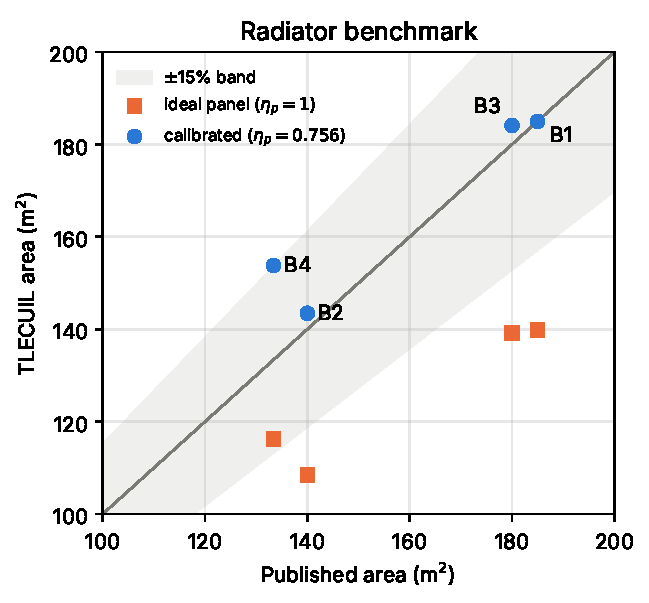
\includegraphics[width=0.48\textwidth]{benchmark_parity.pdf}
\caption{Predicted against published radiator areas. Points on the diagonal agree
exactly. Orange: the ideal panel misses every design low. Blue: one calibrated factor
brings B1--B3 onto the line; B4 sits just outside the $\pm15\%$ band.}
\label{fig:parity}
\end{figure}

With an ideal panel, \tlecuil{} underestimates every design, by
\idealmin--\idealmax\,\%. The effectiveness back-calculated from each of B1, B2 and B3
lies between 0.756 and 0.775. A single, consistent gap points to one systematic factor
rather than scatter. The panel temperature drop and fin efficiency that the ideal model
leaves out (Section~\ref{sec:etap}) are the probable cause, but the sources do not give
enough panel detail to confirm it. With $\eta_p$ from B1 alone, B2 and B3 are predicted
to \errBtwo\,\% and \errBthree\,\%. The sources do not say which sink sized the 2025
radiators. Using 250\,K instead of the 270\,K requirement value changes these to
\sinkBtwo\,\% and \sinkBthree\,\%.

\paragraph{B4 falls outside the band (\errBfour\,\%).} Three features of the source limit
the comparison:
(i)~it does not state whether 133.4\,m$^2$ is planform or total radiating area;
(ii)~it does not state a margin, and adding NASA's usual 10\,\% would raise the
prediction to 169\,m$^2$;
(iii)~its sink is a range (50--220\,K surface, view factor 0.5 to the surface and 0.5
to space) \cite{oleson2022deployable}.
Even with the coldest sink in that range, \tlecuil{} gives 146\,m$^2$ (+10\,\%). The
implied $\eta_p=0.87$ suggests a more effective panel design, consistent with the
different (accordion-deployed) radiator in that concept, rather than an error in the
physics. This is an inference, not something the source states.
\emph{Weak plausibility check:} to match the same concept's equatorial radiator
(216.2\,m$^2$), \tlecuil{} needs an effective sink of about 295\,K. That value is not
excluded by the 100--320\,K equatorial range reported in a different study
\cite{mason2025trades}, but the range is wide enough that this proves little.

\subsection{Electrical chain and first law}
\tablesysbench

The S1 gross output is an identity: the source's 40\,kWe net plus 3\,kWe losses plus
5\,kWe parasitics equals 48\,kWe by construction, so it is not counted as agreement.
All other quantities agree to within 5\,\%.

\emph{The 2\,kWe fixed load is an interpretation.} \textcite{mason2025trades} allow
``up to 2\,kWe'' of housekeeping power, supplied in part by an auxiliary source, and do
not say it is drawn from the converter. The table therefore shows S2 and S3 both with
and without it. With it, gross output matches to within 0.5\,\% and heat load to within
4.3\,\%. Without it, gross output is low by 4--5\,\% and heat load matches to within
3.1\,\%. Both readings pass. The residual heat-load differences are consistent with
reactor and piping losses that the source does not quantify.

\paragraph{Electronics radiator (information only).} With the S2 and S3 inputs (270\,K
sink), \tlecuil{} gives electronics radiator areas of \elecStirling\,m$^2$ (Stirling) and
\elecBrayton\,m$^2$ (Brayton). The published controller plus user-interface radiators
total \elecStirlingPub{} and \elecBraytonPub\,m$^2$ \cite{mason2025trades}. \tlecuil{}
sends \emph{all} PMAD loss and parasitic power to a single 333\,K radiator. The source
does not say how those losses are split among controller electronics, the transmission
cable and other components, and any part not rejected by those radiators would explain
the difference. Treat \tlecuil{}'s electronics radiator as a probable upper bound.

\subsection{Scaling}
\tablescalebench

\emph{Stirling:} without a fixed load, \tlecuil{} under-predicts reactor power at small
sizes ($-15\,\%$ at 10\,kWe). With a 2\,kWe fixed load, it is within 1\,\% from 10 to
100\,kWe, and the efficiency implied by NASA's numbers is then constant (0.286--0.290).
That suggests, but does not prove, that NASA's model carries a size-independent load of
about this magnitude. Radiator areas are within 3\,\% except at 20\,kWe ($-9\,\%$),
which \tlecuil{} does not explain; the source gives no breakdown at that size.

\emph{Brayton:} \tlecuil{} under-predicts at 10\,kWe and over-predicts at 80--100\,kWe.
The ``Implied $\eta$'' column shows why. NASA's numbers imply a Brayton efficiency
that rises from 0.18 at 10\,kWe to 0.22 at 100\,kWe, while \tlecuil{} holds the
40\,kWe value. EZ FSP Sizer derives converter performance from hardware-based
models \cite{mason2025trades}; \tlecuil{} expects the user to supply it. For
100\,kWe Brayton work, the current NASA design point \cite{nasa2025fsp,wilson2026dose},
users should enter a size-appropriate efficiency. The 10\,kWe Brayton point stays
$-10\,\%$ low even with the fixed load.

\subsection{Conversion efficiency}
Table~\ref{tab:carnot} gives the fraction of Carnot implied by each published
efficiency. These values guide the choice of $f_C$ (Section~\ref{sec:eta}). They are not
benchmarks, because each one depends on how its source defines $T_h$ and $T_c$.
\tablecarnot
\FloatBarrier

%=====================================================================
\section{Comparison with the NASA EZ FSP Sizer}\label{sec:ez}
%=====================================================================

\subsection{What EZ FSP Sizer is}
EZ FSP Sizer is a spreadsheet-based nuclear power system sizing tool developed at
NASA Glenn Research Center. It was first built to analyse the Jupiter Icy Moons
Orbiter power system under the Prometheus program, then revised for
Constellation-era FSP studies \cite{mason2025trades,charoenboonvivat2025uq}. It
combines first-order calculations with hardware-based curve fits. It includes
reactor and shield sizing updated with DOE inputs; Brayton and Stirling
thermodynamic models with cycle optimisation; heat rejection with several fluids,
materials and geometries, including transient radiator performance over the lunar
day--night cycle; and PMAD electronics, thermal management and cabling
\cite{mason2025trades}. Its converter mass and performance models derive from the
10.5\,kWe Brayton and 12\,kWe Stirling hardware references \cite{mason2025trades}, and
its masses carry a 20\,\% growth allowance \cite{charoenboonvivat2025uq}. A 2025
framework adds probabilistic uncertainty to its mass estimates
\cite{charoenboonvivat2025uq}.

\begin{review}
This comparison relies on published descriptions only. The author has not had
access to EZ FSP Sizer, and no public user manual was found. The capabilities listed
for it are those stated in \cite{mason2025trades,charoenboonvivat2025uq}.
\end{review}

\subsection{Side-by-side}
\begin{center}
\small
\begin{tabularx}{\textwidth}{>{\raggedright\arraybackslash}p{0.17\textwidth}>{\raggedright\arraybackslash}X>{\raggedright\arraybackslash}X}
\toprule
Aspect & EZ FSP Sizer \cite{mason2025trades,charoenboonvivat2025uq} & \tlecuil{} \\
\midrule
Origin, access & NASA GRC, government tool; published descriptions only & Open source (Python + browser page) \\
Method & First-order physics + hardware-based curve fits; iterative energy balance & First principles only; no curve fits \\
Reactor, shield & Sizing algorithms with DOE inputs & Heat source only; no core or shield model \\
Conversion & Brayton and Stirling cycle models with optimisation & Fixed $\eta$ or fraction of Carnot, user-supplied \\
Heat rejection & Multiple fluids, materials, geometries; day--night transients & Steady state; isothermal or fluid loop (closed form); one sink; calibrated $\eta_p$ \\
PMAD & Electronics, thermal management, cabling & Lumped efficiency + proportional and fixed loads \\
Mass & All subsystems; 20\,\% growth allowance & None (by design) \\
Uncertainty & Separate 2025 framework & None yet; runs fast enough for Monte Carlo \\
Public description & Conference papers and NASA TMs (internal documentation not reviewed here) & This document, code comments, tests, benchmarks \\
Typical use & Government reference designs, architecture trades & Transparent first-order checks, teaching, cross-checking published numbers, thermal power and temperatures as inputs to transport analyses \\
\bottomrule
\end{tabularx}
\end{center}

\subsection{Where \tlecuil{} is stronger}
\begin{itemize}
  \item \textbf{Traceability.} Every equation is derived, cited and tied to a line of
        code and a test. A reviewer can audit it end to end from public sources.
  \item \textbf{Openness and reproducibility.} Anyone can run, check and extend it.
        Results are reproducible from the published inputs listed in
        \texttt{benchmarks.py}.
  \item \textbf{Cross-checking.} Because it shares no correlations with EZ FSP Sizer,
        it can cross-check numbers produced by that tool, within the limits shown in
        Section~\ref{sec:bench}, including the one calibrated factor.
  \item \textbf{Speed and reach.} No size limit; about 5\,$\mu$s per case in Python
        (measured on the development machine), fast enough for Monte Carlo studies;
        runs in a browser. Its thermal power and operating temperatures can feed OpenMC
        or Geant4 models.
\end{itemize}

\subsection{Where \tlecuil{} is weaker}
\begin{itemize}
  \item \textbf{No mass.} The trade NASA actually optimises, total system mass,
        cannot be done in \tlecuil{} yet.
  \item \textbf{No reactor, shield or dose physics.} These dominate mass in published
        designs (the shield is the heaviest single item in \cite{mason2011arch}).
  \item \textbf{Efficiency is an input.} Size-dependent converter performance is
        missing. That causes the Brayton scaling differences above.
  \item \textbf{Calibrated panel.} $\eta_p$ comes from one design; a physical panel model
        would remove that dependence.
  \item \textbf{Steady state, one sink.} No day--night transient, view-factor or terrain
        model.
\end{itemize}

\subsection{Verdict}
Neither tool replaces the other. For design decisions that depend on mass, EZ FSP
Sizer is the better tool, because it carries hardware-based mass and performance
models that \tlecuil{} deliberately omits. For a transparent, reviewable first-order
balance, cross-checking published numbers, teaching, and supplying first-order inputs
to higher-fidelity reactor and shielding analyses, \tlecuil{} is the better fit.

%=====================================================================
\section{Moon versus Mars}\label{sec:mars}
%=====================================================================
NASA's FSP technology is intended to work on both the Moon and Mars, with design
changes not expected to be significant for the environmental differences studied
\cite{fsp2010icd,poston2011mars}. For a radiator sizer the key differences are:
\begin{itemize}
  \item \textbf{Sink temperature.} An early NASA review gave lunar effective sinks of
        221--325\,K, depending on radiator orientation and properties, and
        preliminary Mars values of 175--250\,K \cite{perezdavis1992env}. The 2025
        government study gives 100--200\,K (south pole) and 100--320\,K (equator) for
        a fixed vertical radiator on the Moon \cite{mason2025trades}. In \tlecuil{},
        the user sets $T_s$ for the site.
  \item \textbf{Convection.} Mars's thin CO$_2$ atmosphere allows convective heat
        rejection. One study estimated that a forced-convection heat exchanger could
        cut the optimal cycle mass of a 40\,kWe Mars system by 80\,\% compared with a
        radiator \cite{colgan_marsconvection}. \tlecuil{} models radiation only, so
        its Mars radiator areas are conservative (too large).
  \item \textbf{Dust.} Wind-blown dust can coat and abrade radiator surfaces on Mars
        \cite{gaier1991dust,perezdavis1992env}. In \tlecuil{} this enters only through
        a lower end-of-life emissivity.
\end{itemize}

%=====================================================================
\section{Limitations and future work}\label{sec:limits}
%=====================================================================
\begin{enumerate}
  \item \textbf{Mass module} built on cited specific masses. Published design data
        allow derived values, for example a heat-rejection subsystem of 701\,kg for
        140\,m$^2$ ($\approx5.0$\,kg/m$^2$) in the 2025 Stirling design
        \cite{mason2025trades}. Uncertainty should follow
        \cite{charoenboonvivat2025uq}.
  \item \textbf{Physical panel model} (heat-pipe $\Delta T$, fin equation) to replace
        the calibrated $\eta_p$.
  \item \textbf{Size-dependent converter efficiency} maps for Brayton and Stirling.
  \item \textbf{PMAD loss allocation} between local electronics, cable and remote
        electronics, to remove the conservative bias in the electronics radiator.
  \item \textbf{Environment}: view factors to terrain, solar loading, day--night
        cycle; Mars convection and dust.
  \item \textbf{Shielding and dose} from transport results (OpenMC, MCNP, Geant4).
  \item \textbf{Uncertainty quantification} by Monte Carlo over input distributions.
\end{enumerate}

%=====================================================================
\section{Reproducibility}
%=====================================================================
\begin{verbatim}
python -m pytest -q          # 16 verification and benchmark tests
python benchmarks.py         # regenerates docs/benchmark_tables.tex
cd docs && python make_figures.py   # regenerates the figures
python tlecuil.py --power 100
cd docs && latexmk -pdf tlecuil_theory.tex
\end{verbatim}
The HTML page re-implements the same engine in JavaScript.
\texttt{check\_parity.js} compares it with the Python output on reference cases;
the two must agree to machine precision.

\appendix
%=====================================================================
\section{Physics and mathematics review checklist}
%=====================================================================
\begin{center}
\small
\begin{tabularx}{\textwidth}{lXX}
\toprule
Equation & Basis & Independent check \\
\midrule
\eqref{eq:ppar}--\eqref{eq:lpmad} & Power bookkeeping & S1--S3 (S1 gross is an identity) \\
\eqref{eq:firstlaw}--\eqref{eq:qin} & First law, steady state & Hand calculation test \\
\eqref{eq:carnot} & Second law \cite{smith2001thermo} & Guard rejects $\eta>\eta_C$ \\
\eqref{eq:fc} & Modelling assumption & Table~\ref{tab:carnot} spread \\
\eqref{eq:loss} & Bookkeeping; data in \cite{oleson2022deployable} & Implementation check only (residual) \\
\eqref{eq:flux} & Stefan--Boltzmann, gray diffuse \cite{howell2021radiation} & Hand calculation test \\
\eqref{eq:planform} & Definition \cite{fsp2010icd,mason2025trades} & Regression test (v0.1 error) \\
\eqref{eq:k} & Fin-efficiency factor \cite{wang2021entropy,gilmore2002thermal} & B1 calibration, B2--B4 prediction \\
\eqref{eq:afluid}--\eqref{eq:series} & Energy balance on a strip; partial fractions; series & SciPy quadrature, sinks $10^{-9}$--290\,K; isothermal limit \\
\eqref{eq:balance} & Algebraic consequence of the above & Implementation check (residual $<10^{-9}$) \\
\eqref{eq:mf} & 200\,MeV per fission \cite{lamarsh2017} & 1.05\,g/MWd rule \\
\eqref{eq:tauopt} & Calculus; 3/4 limit \cite{bucher1960}; 0.75--0.80 \cite{wetch1988mcnsps} & Golden-section search \\
\bottomrule
\end{tabularx}
\end{center}

%=====================================================================
\section{Answers to the Try it exercises}\label{app:answers}
%=====================================================================
\begin{description}
  \item[\ref{try:pconv}] $\Pconv = (100/0.90 + 2)/1 = 113.1$\,kWe. PMAD receives $113.1-2 = 111.1$\,kWe
        and delivers 100\,kWe, so it loses 11.1\,kW.
  \item[\ref{try:eta}] $(1-\eta)/\eta$: 4.0\,kW per kWe at $\eta=0.20$, and 2.33\,kW per kWe at
        $\eta=0.30$. The heat load falls by a factor of $4.0/2.33=1.71$.
  \item[\ref{try:rad}] Flux $=0.85\,\sigma T^4$: 1234\,W/m$^2$ at 400\,K, so $A=81.0$\,m$^2$; and
        3012\,W/m$^2$ at 500\,K, so $A=33.2$\,m$^2$. The ratio is $(500/400)^4=2.44$.
  \item[\ref{try:fuel}] $400\times10^{-3}\times3652.5=1461$\,MWd, so $m_f\approx1461\times1.05\text{ g}\approx1.53$\,kg.
  \item[\ref{try:opt}] With $f_C=1$: $4\tau^2-3\tau=0$, so $\tau=3/4$ (the root $\tau=0$ is not
        physical). Check: $1/(3/4)+1/(1/4)-4/(3/4)=4/3+4-16/3=0$.
\end{description}

%=====================================================================
\section{Glossary}\label{app:glossary}
%=====================================================================
\begin{description}
  \item[Benchmark] A comparison of a model with another model or a published design.
  \item[Brayton cycle] A gas-turbine heat engine: compress a gas, heat it, expand it
        through a turbine.
  \item[Carnot efficiency] The highest efficiency any heat engine can have between two
        temperatures, $1-T_c/T_h$.
  \item[Effective sink temperature] The single temperature that represents everything
        the radiator sees (sky, ground, Sun).
  \item[Emissivity] How well a surface radiates compared with a perfect black body
        (0 to 1).
  \item[Fin efficiency] How much heat a panel actually radiates compared with an ideal
        panel held at the base temperature.
  \item[First-order model] A model that keeps only the physics that dominates the answer.
  \item[Fission] Splitting a heavy nucleus such as U-235, releasing about 200\,MeV.
  \item[Heat pipe] A sealed tube that moves heat by evaporating and condensing a fluid,
        with little temperature drop.
  \item[kWe, kWt] Kilowatts of electrical and of thermal power.
  \item[Margin] Extra capacity added on purpose to cover uncertainty.
  \item[Parasitic load] Electricity the plant uses itself (pumps, controls).
  \item[Planform area] The size of a panel as built, seen from the front.
  \item[PMAD] Power management and distribution: electronics and cables between the
        converter and the users.
  \item[Radiating area] The total surface that emits heat. A two-sided panel has twice
        its planform area.
  \item[Stirling engine] A sealed piston engine that runs on an external heat source.
  \item[Validation] Checking a model against measurements of reality.
  \item[Verification] Checking that the code solves the model's equations correctly.
\end{description}

%=====================================================================
\section{Nomenclature}
%=====================================================================
\begin{longtable}{>{$}l<{$}p{0.5\textwidth}l}
\toprule
\text{Symbol} & Meaning & Unit\\
\midrule
\Pdel & Power delivered to the user bus & kWe\\
\Pconv & Gross converter electrical output & kWe\\
\Pth & Reactor thermal power & kWt\\
Q_\text{in} & Heat delivered to the converter & kWt\\
Q_\text{conv} & Heat rejected by the converter (main radiator load) & kW\\
Q_\text{elec} & Electronics heat & kW\\
Q_\text{loss} & Reactor and piping heat loss & kW\\
P_\text{par}, P_\text{fix} & Parasitic load; fixed part & kWe\\
L_\text{PMAD} & PMAD loss & kW\\
f_\text{par}, f_\text{loss} & Proportional parasitic fraction; reactor loss fraction & --\\
\eta, \eta_C, f_C & Conversion efficiency; Carnot efficiency; fraction of Carnot & --\\
\eta_\text{PMAD} & PMAD efficiency & --\\
\eta_p & Panel effectiveness & --\\
T_h, T_c & Converter hot and cold temperatures & K\\
T_\text{in}, T_\text{out}, T_s, T_e & Radiator inlet, outlet; sink; electronics radiator & K\\
\varepsilon, \sigma & Emissivity; Stefan--Boltzmann constant & --; \si{W.m^{-2}.K^{-4}}\\
m & Area margin & --\\
A, A_\text{planform} & Total radiating area; panel planform & m$^2$\\
\dot m c_p & Coolant heat-capacity rate & W/K\\
E_f, m_f & Energy per fission; U-235 fissioned & MeV; kg\\
\bottomrule
\end{longtable}

\setcounter{biburlnumpenalty}{9000}\setcounter{biburllcpenalty}{7000}\setcounter{biburlucpenalty}{8000}
\printbibliography[heading=bibintoc]
\end{document}
